\documentclass[twoside]{book}

% Packages required by doxygen
\usepackage{calc}
\usepackage{doxygen}
\usepackage{graphicx}
\usepackage[utf8]{inputenc}
\usepackage{makeidx}
\usepackage{multicol}
\usepackage{multirow}
\usepackage{textcomp}
\usepackage[table]{xcolor}

% Font selection
\usepackage[T1]{fontenc}
\usepackage{mathptmx}
\usepackage[scaled=.90]{helvet}
\usepackage{courier}
\usepackage{amssymb}
\usepackage{sectsty}
\renewcommand{\familydefault}{\sfdefault}
\allsectionsfont{%
  \fontseries{bc}\selectfont%
  \color{darkgray}%
}
\renewcommand{\DoxyLabelFont}{%
  \fontseries{bc}\selectfont%
  \color{darkgray}%
}

% Page & text layout
\usepackage{geometry}
\geometry{%
  a4paper,%
  top=2.5cm,%
  bottom=2.5cm,%
  left=2.5cm,%
  right=2.5cm%
}
\tolerance=750
\hfuzz=15pt
\hbadness=750
\setlength{\emergencystretch}{15pt}
\setlength{\parindent}{0cm}
\setlength{\parskip}{0.2cm}
\makeatletter
\renewcommand{\paragraph}{%
  \@startsection{paragraph}{4}{0ex}{-1.0ex}{1.0ex}{%
    \normalfont\normalsize\bfseries\SS@parafont%
  }%
}
\renewcommand{\subparagraph}{%
  \@startsection{subparagraph}{5}{0ex}{-1.0ex}{1.0ex}{%
    \normalfont\normalsize\bfseries\SS@subparafont%
  }%
}
\makeatother

% Headers & footers
\usepackage{fancyhdr}
\pagestyle{fancyplain}
\fancyhead[LE]{\fancyplain{}{\bfseries\thepage}}
\fancyhead[CE]{\fancyplain{}{}}
\fancyhead[RE]{\fancyplain{}{\bfseries\leftmark}}
\fancyhead[LO]{\fancyplain{}{\bfseries\rightmark}}
\fancyhead[CO]{\fancyplain{}{}}
\fancyhead[RO]{\fancyplain{}{\bfseries\thepage}}
\fancyfoot[LE]{\fancyplain{}{}}
\fancyfoot[CE]{\fancyplain{}{}}
\fancyfoot[RE]{\fancyplain{}{\bfseries\scriptsize Generated on Sat Mar 24 2018 16\-:07\-:26 for My Project by Doxygen }}
\fancyfoot[LO]{\fancyplain{}{\bfseries\scriptsize Generated on Sat Mar 24 2018 16\-:07\-:26 for My Project by Doxygen }}
\fancyfoot[CO]{\fancyplain{}{}}
\fancyfoot[RO]{\fancyplain{}{}}
\renewcommand{\footrulewidth}{0.4pt}
\renewcommand{\chaptermark}[1]{%
  \markboth{#1}{}%
}
\renewcommand{\sectionmark}[1]{%
  \markright{\thesection\ #1}%
}

% Indices & bibliography
\usepackage{natbib}
\usepackage[titles]{tocloft}
\setcounter{tocdepth}{3}
\setcounter{secnumdepth}{5}
\makeindex

% Custom commands
\newcommand{\clearemptydoublepage}{%
  \newpage{\pagestyle{empty}\cleardoublepage}%
}


%===== C O N T E N T S =====

\begin{document}

% Titlepage & ToC
\pagenumbering{roman}
\begin{titlepage}
\vspace*{7cm}
\begin{center}%
{\Large My Project }\\
\vspace*{1cm}
{\large Generated by Doxygen 1.8.6}\\
\vspace*{0.5cm}
{\small Sat Mar 24 2018 16:07:26}\\
\end{center}
\end{titlepage}
\clearemptydoublepage
\tableofcontents
\clearemptydoublepage
\pagenumbering{arabic}

%--- Begin generated contents ---
\chapter{My Main Page usig markdown}
\label{index}{\tt http\-://www.\-stack.\-nl/$\sim$dimitri/doxygen/manual/markdown.\-html}

{\tt https\-://segmentfault.\-com/markdown}


\begin{DoxyEnumerate}
\item 列出所有元素:
\begin{DoxyItemize}
\item 无序列表元素 \doxyref{A}{p.}{class_a}
\begin{DoxyEnumerate}
\item 元素 \doxyref{A}{p.}{class_a} 的有序子列表
\end{DoxyEnumerate}
\item 前面加四个空格
\end{DoxyItemize}
\item 列表里的多段换行: 前面必须加四个空格, 这样换行,整体的格式不会乱
\item 列表里引用:

$>$ 前面空一行 $>$ 仍然需要在 $>$ 前面加四个空格
\item 列表里代码段:

{\ttfamily  前面四个空格,之后按代码语法} 书写 ``` \begin{DoxyVerb}或者直接空八个,引入代码块
\end{DoxyVerb}

\end{DoxyEnumerate}

公式 当你需要在编辑器中插入数学公式时,可以使用两个美元符 \$\$ 包裹 Te\-X 或 La\-Te\-X 格式的数学公式来实现。提交后,问答和文章页会根据需要加载 Mathjax 对数学公式进行渲染。如:

\$\$ x = \{-\/b  \{b$^\wedge$2-\/4ac\}  2a\}. \$\$

\$\$ x \{why-\/equal.\-html\}\{=\} y$^\wedge$2 + 1 \$\$

同时也支持 H\-T\-M\-L 属性,如:

{\tt https\-://www.\-jianshu.\-com/p/888c5eaebabd}

方法三:使用\-Math\-Jax引擎 大家都看过\-Stackoverflow上的公式吧,漂亮,其生成的不是图片。这就要用到\-Math\-Jax引擎,在\-Markdown中添加\-Math\-Jax引擎也很简单,

\$\$x=\{-\/b\{b$^\wedge$2-\/4ac\}\}\{2a\}\$\$\textbackslash{}(x=\{-\/b\{b$^\wedge$2-\/4ac\}\}\{2a\}\textbackslash{})

然后,再使用\-Tex写公式。\$\$公式\$\$ 表示行间公式,本来\-Tex中使用(公式) 表示行内公式,但因为\-Markdown中 是转义字符,所以在\-Markdown中输入行内公式使用(公式) ,如下代码:

\$\$x=\{-\/b\{b$^\wedge$2-\/4ac\}\}\{2a\}\$\$\textbackslash{}(x=\{-\/b\{b$^\wedge$2-\/4ac\}\}\{2a\}\textbackslash{})

dd

\begin{TabularC}{2}
\hline
\rowcolor{lightgray}{\bf First Header }&{\bf Second Header  }\\\cline{1-2}
Content Cell &Content Cell \\\cline{1-2}
Content Cell &Content Cell \\\cline{1-2}
\end{TabularC}
block-\/level H\-T\-M\-L elements — e.\-g. , \begin{TabularC}{0}
\hline
\end{TabularC}

\begin{DoxyPre}, \end{DoxyPre}



\begin{DoxyPre}, etc. — must be separated from surrounding content by blank lines, and the start and end tags of the block should not be indented with tabs or spaces.\end{DoxyPre}



\begin{DoxyPre}Here is text for one paragraph.\end{DoxyPre}



\begin{DoxyPre}We continue with more text in another paragraph.\end{DoxyPre}



\begin{DoxyPre}\section*{This is a level 1 header
}\end{DoxyPre}



\begin{DoxyPre}\end{DoxyPre}



\begin{DoxyPre}\subsection*{This is a level 2 header
}\end{DoxyPre}



\begin{DoxyPre}\end{DoxyPre}



\begin{DoxyPre}\section*{This is a level 1 header}\end{DoxyPre}



\begin{DoxyPre}\end{DoxyPre}



\begin{DoxyPre}\subsubsection*{This is level 3 header}\end{DoxyPre}



\begin{DoxyPre}\end{DoxyPre}



\begin{DoxyPre}\begin{quotation}
This is a block quote
spanning multiple lines

\end{quotation}
\end{DoxyPre}



\begin{DoxyPre}0  if OK\par
>1 if NOK\end{DoxyPre}



\begin{DoxyPre}
\begin{DoxyItemize}
\item Item 1

More text for this item.
\end{DoxyItemize}\end{DoxyPre}



\begin{DoxyPre}
\begin{DoxyItemize}
\item Item 2
  + nested list item.
  + another nested item.
\item Item 3
\end{DoxyItemize}\end{DoxyPre}



\begin{DoxyPre}{\tt The link text}
{\tt The link text}
{\tt The link text} 
{\tt The link text}\end{DoxyPre}



\begin{DoxyPre}\begin{TabularC}{3}
\hline
\rowcolor{lightgray}\PBS\raggedleft {\bf Right }&\PBS\centering {\bf Center }&{\bf Left  

}\\\cline{1-3}
\PBS\raggedleft 10    &\PBS\centering 10     &10    
\\\cline{1-3}
\PBS\raggedleft 1000  &\PBS\centering 1000   &1000  
\\\cline{1-3}
\end{TabularC}
\end{DoxyPre}



\begin{DoxyPre}\begin{TabularC}{3}
\hline
\rowcolor{lightgray}\PBS\raggedleft {\bf Right }&\PBS\centering {\bf Center }&{\bf Left  

}\\\cline{1-3}
\PBS\raggedleft 10    &\PBS\centering 10     &10    
\\\cline{1-3}
\PBS\raggedleft 1000  &\PBS\centering \\\cline{1-3}
\end{TabularC}
\end{DoxyPre}
\section{Header 1                }\label{index_labelid}

\begin{DoxyPre}\end{DoxyPre}



\begin{DoxyPre}\end{DoxyPre}
\subsection{Header 2}\label{index_labelid2}

\begin{DoxyPre}
text\end{DoxyPre}



\begin{DoxyPre} text\end{DoxyPre}



\begin{DoxyPre}  text\end{DoxyPre}



\begin{DoxyPre}   code
\end{DoxyPre}

\chapter{Hierarchical Index}
\section{Class Hierarchy}
This inheritance list is sorted roughly, but not completely, alphabetically\-:\begin{DoxyCompactList}
\item \contentsline{section}{A}{\pageref{class_a}}{}
\begin{DoxyCompactList}
\item \contentsline{section}{C}{\pageref{class_c}}{}
\item \contentsline{section}{D}{\pageref{class_d}}{}
\begin{DoxyCompactList}
\item \contentsline{section}{E}{\pageref{class_e}}{}
\end{DoxyCompactList}
\end{DoxyCompactList}
\item \contentsline{section}{B}{\pageref{class_b}}{}
\begin{DoxyCompactList}
\item \contentsline{section}{D}{\pageref{class_d}}{}
\end{DoxyCompactList}
\end{DoxyCompactList}

\chapter{Class Index}
\section{Class List}
Here are the classes, structs, unions and interfaces with brief descriptions\-:\begin{DoxyCompactList}
\item\contentsline{section}{{\bf A} }{\pageref{class_a}}{}
\item\contentsline{section}{{\bf B} }{\pageref{class_b}}{}
\item\contentsline{section}{{\bf C} }{\pageref{class_c}}{}
\item\contentsline{section}{{\bf D} }{\pageref{class_d}}{}
\item\contentsline{section}{{\bf E} }{\pageref{class_e}}{}
\end{DoxyCompactList}

\chapter{File Index}
\section{File List}
Here is a list of all files with brief descriptions\-:\begin{DoxyCompactList}
\item\contentsline{section}{/home/haijunz/13301338176-\/ml/\-Python\-\_\-\-C++\-\_\-caffe-\/tfskills-\/android/call-\/graph-\/valgrind/static-\/doxy/{\bf diagrams\-\_\-a.\-h} }{\pageref{diagrams__a_8h}}{}
\item\contentsline{section}{/home/haijunz/13301338176-\/ml/\-Python\-\_\-\-C++\-\_\-caffe-\/tfskills-\/android/call-\/graph-\/valgrind/static-\/doxy/{\bf diagrams\-\_\-b.\-h} }{\pageref{diagrams__b_8h}}{}
\item\contentsline{section}{/home/haijunz/13301338176-\/ml/\-Python\-\_\-\-C++\-\_\-caffe-\/tfskills-\/android/call-\/graph-\/valgrind/static-\/doxy/{\bf diagrams\-\_\-c.\-h} }{\pageref{diagrams__c_8h}}{}
\item\contentsline{section}{/home/haijunz/13301338176-\/ml/\-Python\-\_\-\-C++\-\_\-caffe-\/tfskills-\/android/call-\/graph-\/valgrind/static-\/doxy/{\bf diagrams\-\_\-d.\-h} }{\pageref{diagrams__d_8h}}{}
\item\contentsline{section}{/home/haijunz/13301338176-\/ml/\-Python\-\_\-\-C++\-\_\-caffe-\/tfskills-\/android/call-\/graph-\/valgrind/static-\/doxy/{\bf diagrams\-\_\-e.\-h} }{\pageref{diagrams__e_8h}}{}
\end{DoxyCompactList}

\chapter{Class Documentation}
\section{A Class Reference}
\label{class_a}\index{A@{A}}


{\ttfamily \#include $<$diagrams\-\_\-a.\-h$>$}



Inheritance diagram for A\-:\nopagebreak
\begin{figure}[H]
\begin{center}
\leavevmode
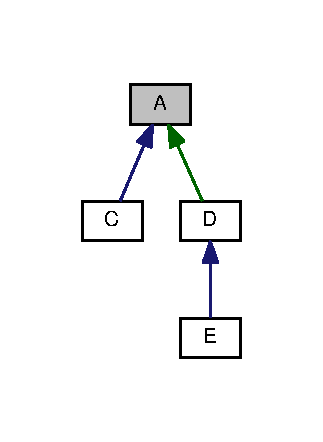
\includegraphics[width=155pt]{class_a__inherit__graph}
\end{center}
\end{figure}


Collaboration diagram for A\-:\nopagebreak
\begin{figure}[H]
\begin{center}
\leavevmode
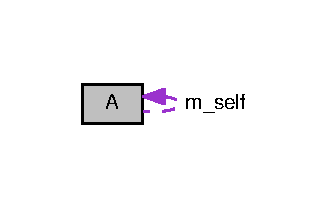
\includegraphics[width=159pt]{class_a__coll__graph}
\end{center}
\end{figure}
\subsection*{Public Attributes}
\begin{DoxyCompactItemize}
\item 
{\bf A} $\ast$ {\bf m\-\_\-self}
\end{DoxyCompactItemize}


\subsection{Detailed Description}


Definition at line 5 of file diagrams\-\_\-a.\-h.



\subsection{Member Data Documentation}
\index{A@{A}!m\-\_\-self@{m\-\_\-self}}
\index{m\-\_\-self@{m\-\_\-self}!A@{A}}
\subsubsection[{m\-\_\-self}]{\setlength{\rightskip}{0pt plus 5cm}{\bf A}$\ast$ A\-::m\-\_\-self}\label{class_a_a086d3a4efc697dba0601b9fef3d082ad}


Definition at line 6 of file diagrams\-\_\-a.\-h.



The documentation for this class was generated from the following file\-:\begin{DoxyCompactItemize}
\item 
/home/haijunz/13301338176-\/ml/\-Python\-\_\-\-C++\-\_\-caffe-\/tfskills-\/android/call-\/graph-\/valgrind/static-\/doxy/{\bf diagrams\-\_\-a.\-h}\end{DoxyCompactItemize}

\section{B Class Reference}
\label{class_b}\index{B@{B}}


{\ttfamily \#include $<$diagrams\-\_\-b.\-h$>$}



Inheritance diagram for B\-:\nopagebreak
\begin{figure}[H]
\begin{center}
\leavevmode
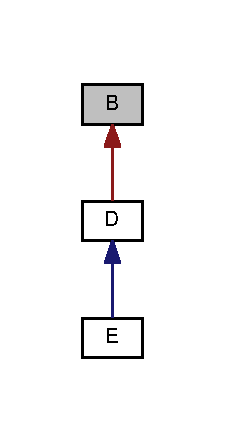
\includegraphics[width=108pt]{class_b__inherit__graph}
\end{center}
\end{figure}


Collaboration diagram for B\-:\nopagebreak
\begin{figure}[H]
\begin{center}
\leavevmode
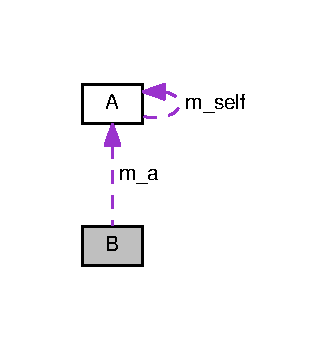
\includegraphics[width=159pt]{class_b__coll__graph}
\end{center}
\end{figure}
\subsection*{Public Attributes}
\begin{DoxyCompactItemize}
\item 
{\bf A} $\ast$ {\bf m\-\_\-a}
\end{DoxyCompactItemize}


\subsection{Detailed Description}


Definition at line 4 of file diagrams\-\_\-b.\-h.



\subsection{Member Data Documentation}
\index{B@{B}!m\-\_\-a@{m\-\_\-a}}
\index{m\-\_\-a@{m\-\_\-a}!B@{B}}
\subsubsection[{m\-\_\-a}]{\setlength{\rightskip}{0pt plus 5cm}{\bf A}$\ast$ B\-::m\-\_\-a}\label{class_b_a26c70b64fe7cf17fcced7755ecff7537}


Definition at line 4 of file diagrams\-\_\-b.\-h.



The documentation for this class was generated from the following file\-:\begin{DoxyCompactItemize}
\item 
/home/haijunz/13301338176-\/ml/\-Python\-\_\-\-C++\-\_\-caffe-\/tfskills-\/android/call-\/graph-\/valgrind/static-\/doxy/{\bf diagrams\-\_\-b.\-h}\end{DoxyCompactItemize}

\section{C Class Reference}
\label{class_c}\index{C@{C}}


{\ttfamily \#include $<$diagrams\-\_\-c.\-h$>$}



Inheritance diagram for C\-:\nopagebreak
\begin{figure}[H]
\begin{center}
\leavevmode
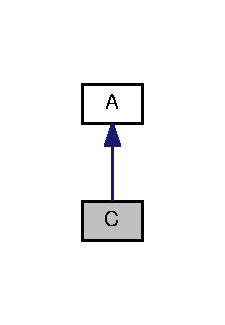
\includegraphics[width=108pt]{class_c__inherit__graph}
\end{center}
\end{figure}


Collaboration diagram for C\-:\nopagebreak
\begin{figure}[H]
\begin{center}
\leavevmode
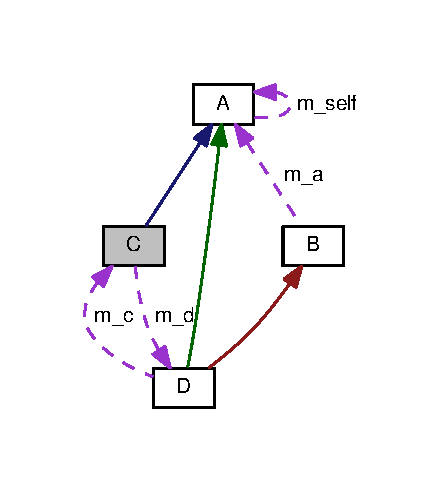
\includegraphics[width=212pt]{class_c__coll__graph}
\end{center}
\end{figure}
\subsection*{Public Attributes}
\begin{DoxyCompactItemize}
\item 
{\bf D} $\ast$ {\bf m\-\_\-d}
\end{DoxyCompactItemize}


\subsection{Detailed Description}


Definition at line 5 of file diagrams\-\_\-c.\-h.



\subsection{Member Data Documentation}
\index{C@{C}!m\-\_\-d@{m\-\_\-d}}
\index{m\-\_\-d@{m\-\_\-d}!C@{C}}
\subsubsection[{m\-\_\-d}]{\setlength{\rightskip}{0pt plus 5cm}{\bf D}$\ast$ C\-::m\-\_\-d}\label{class_c_a4ef972d28b73ff78eba3ab4f54c3b449}


Definition at line 5 of file diagrams\-\_\-c.\-h.



The documentation for this class was generated from the following file\-:\begin{DoxyCompactItemize}
\item 
/home/haijunz/13301338176-\/ml/\-Python\-\_\-\-C++\-\_\-caffe-\/tfskills-\/android/call-\/graph-\/valgrind/static-\/doxy/{\bf diagrams\-\_\-c.\-h}\end{DoxyCompactItemize}

\section{D Class Reference}
\label{class_d}\index{D@{D}}


{\ttfamily \#include $<$diagrams\-\_\-d.\-h$>$}



Inheritance diagram for D\-:\nopagebreak
\begin{figure}[H]
\begin{center}
\leavevmode
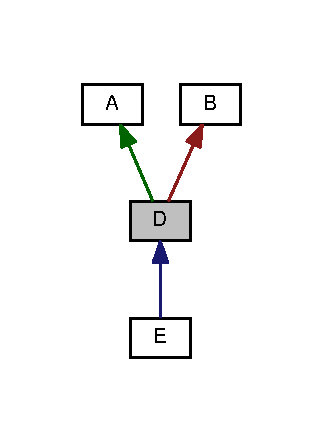
\includegraphics[width=155pt]{class_d__inherit__graph}
\end{center}
\end{figure}


Collaboration diagram for D\-:\nopagebreak
\begin{figure}[H]
\begin{center}
\leavevmode
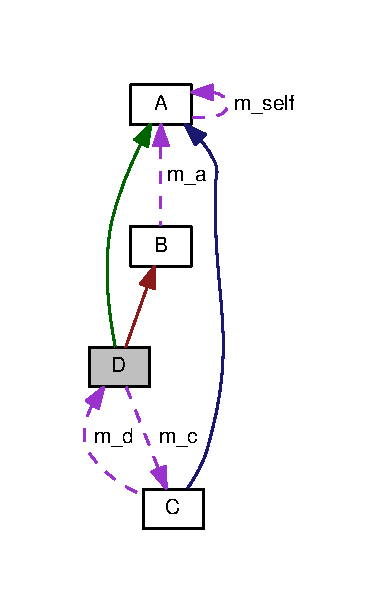
\includegraphics[width=183pt]{class_d__coll__graph}
\end{center}
\end{figure}
\subsection*{Public Attributes}
\begin{DoxyCompactItemize}
\item 
{\bf C} {\bf m\-\_\-c}
\end{DoxyCompactItemize}
\subsection*{Additional Inherited Members}


\subsection{Detailed Description}


Definition at line 6 of file diagrams\-\_\-d.\-h.



\subsection{Member Data Documentation}
\index{D@{D}!m\-\_\-c@{m\-\_\-c}}
\index{m\-\_\-c@{m\-\_\-c}!D@{D}}
\subsubsection[{m\-\_\-c}]{\setlength{\rightskip}{0pt plus 5cm}{\bf C} D\-::m\-\_\-c}\label{class_d_a9d877c7aa092f423f2a073f3c62fef9c}


Definition at line 6 of file diagrams\-\_\-d.\-h.



The documentation for this class was generated from the following file\-:\begin{DoxyCompactItemize}
\item 
/home/haijunz/13301338176-\/ml/\-Python\-\_\-\-C++\-\_\-caffe-\/tfskills-\/android/call-\/graph-\/valgrind/static-\/doxy/{\bf diagrams\-\_\-d.\-h}\end{DoxyCompactItemize}

\section{E Class Reference}
\label{class_e}\index{E@{E}}


{\ttfamily \#include $<$diagrams\-\_\-e.\-h$>$}



Inheritance diagram for E\-:\nopagebreak
\begin{figure}[H]
\begin{center}
\leavevmode
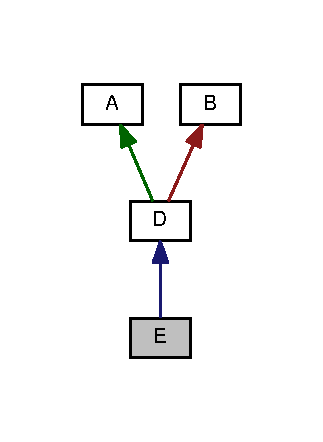
\includegraphics[width=155pt]{class_e__inherit__graph}
\end{center}
\end{figure}


Collaboration diagram for E\-:\nopagebreak
\begin{figure}[H]
\begin{center}
\leavevmode
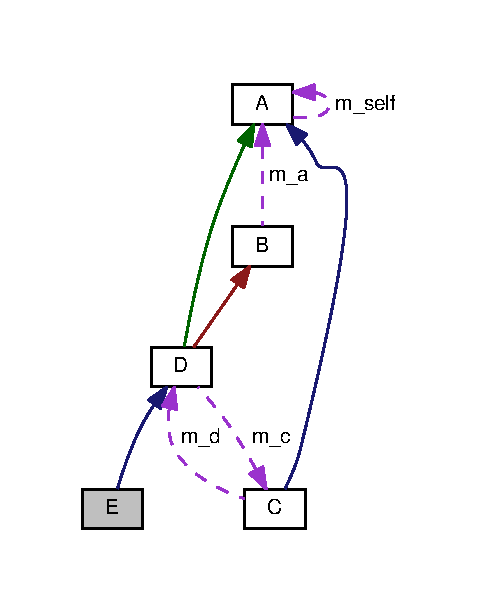
\includegraphics[width=231pt]{class_e__coll__graph}
\end{center}
\end{figure}
\subsection*{Additional Inherited Members}


\subsection{Detailed Description}


Definition at line 5 of file diagrams\-\_\-e.\-h.



The documentation for this class was generated from the following file\-:\begin{DoxyCompactItemize}
\item 
/home/haijunz/13301338176-\/ml/\-Python\-\_\-\-C++\-\_\-caffe-\/tfskills-\/android/call-\/graph-\/valgrind/static-\/doxy/{\bf diagrams\-\_\-e.\-h}\end{DoxyCompactItemize}

\chapter{File Documentation}
\section{/home/haijunz/13301338176-\/ml/\-Python\-\_\-\-C++\-\_\-caffe-\/tfskills-\/android/call-\/graph-\/valgrind/static-\/doxy/diagrams\-\_\-a.h File Reference}
\label{diagrams__a_8h}\index{/home/haijunz/13301338176-\/ml/\-Python\-\_\-\-C++\-\_\-caffe-\/tfskills-\/android/call-\/graph-\/valgrind/static-\/doxy/diagrams\-\_\-a.\-h@{/home/haijunz/13301338176-\/ml/\-Python\-\_\-\-C++\-\_\-caffe-\/tfskills-\/android/call-\/graph-\/valgrind/static-\/doxy/diagrams\-\_\-a.\-h}}
This graph shows which files directly or indirectly include this file\-:\nopagebreak
\begin{figure}[H]
\begin{center}
\leavevmode
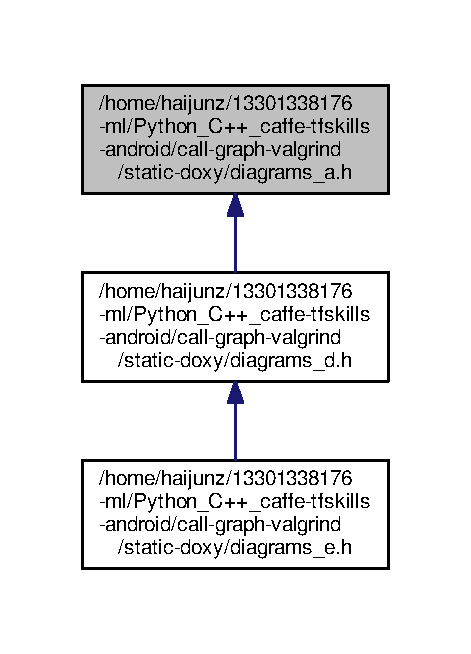
\includegraphics[width=226pt]{diagrams__a_8h__dep__incl}
\end{center}
\end{figure}
\subsection*{Classes}
\begin{DoxyCompactItemize}
\item 
class {\bf A}
\end{DoxyCompactItemize}

\section{/home/haijunz/13301338176-\/ml/\-Python\-\_\-\-C++\-\_\-caffe-\/tfskills-\/android/call-\/graph-\/valgrind/static-\/doxy/diagrams\-\_\-b.h File Reference}
\label{diagrams__b_8h}\index{/home/haijunz/13301338176-\/ml/\-Python\-\_\-\-C++\-\_\-caffe-\/tfskills-\/android/call-\/graph-\/valgrind/static-\/doxy/diagrams\-\_\-b.\-h@{/home/haijunz/13301338176-\/ml/\-Python\-\_\-\-C++\-\_\-caffe-\/tfskills-\/android/call-\/graph-\/valgrind/static-\/doxy/diagrams\-\_\-b.\-h}}
This graph shows which files directly or indirectly include this file\-:\nopagebreak
\begin{figure}[H]
\begin{center}
\leavevmode
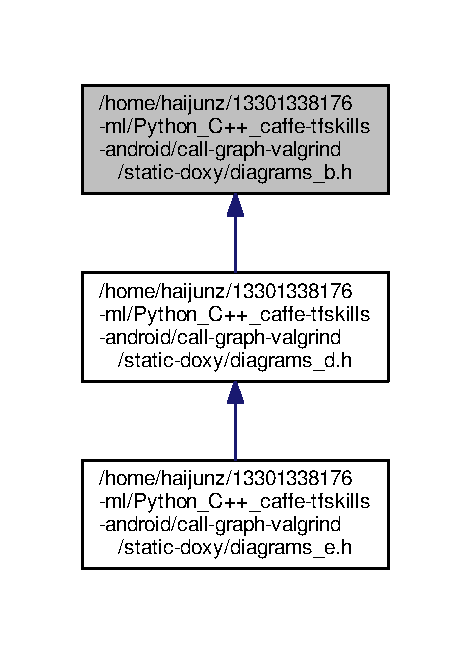
\includegraphics[width=226pt]{diagrams__b_8h__dep__incl}
\end{center}
\end{figure}
\subsection*{Classes}
\begin{DoxyCompactItemize}
\item 
class {\bf B}
\end{DoxyCompactItemize}

\section{/home/haijunz/13301338176-\/ml/\-Python\-\_\-\-C++\-\_\-caffe-\/tfskills-\/android/call-\/graph-\/valgrind/static-\/doxy/diagrams\-\_\-c.h File Reference}
\label{diagrams__c_8h}\index{/home/haijunz/13301338176-\/ml/\-Python\-\_\-\-C++\-\_\-caffe-\/tfskills-\/android/call-\/graph-\/valgrind/static-\/doxy/diagrams\-\_\-c.\-h@{/home/haijunz/13301338176-\/ml/\-Python\-\_\-\-C++\-\_\-caffe-\/tfskills-\/android/call-\/graph-\/valgrind/static-\/doxy/diagrams\-\_\-c.\-h}}
{\ttfamily \#include \char`\"{}diagrams\-\_\-c.\-h\char`\"{}}\\*
Include dependency graph for diagrams\-\_\-c.\-h\-:\nopagebreak
\begin{figure}[H]
\begin{center}
\leavevmode
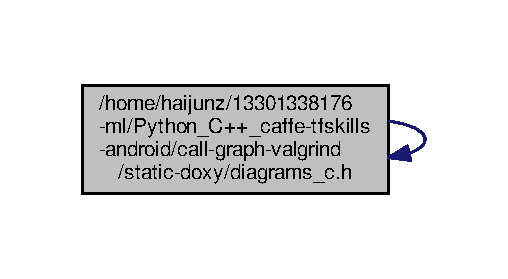
\includegraphics[width=244pt]{diagrams__c_8h__incl}
\end{center}
\end{figure}
This graph shows which files directly or indirectly include this file\-:\nopagebreak
\begin{figure}[H]
\begin{center}
\leavevmode
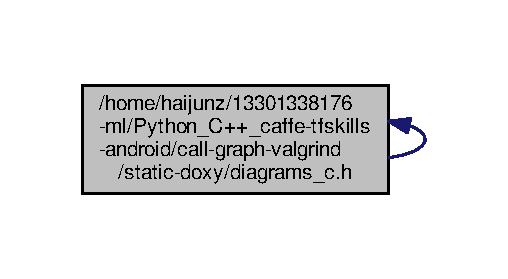
\includegraphics[width=244pt]{diagrams__c_8h__dep__incl}
\end{center}
\end{figure}
\subsection*{Classes}
\begin{DoxyCompactItemize}
\item 
class {\bf C}
\end{DoxyCompactItemize}

\section{/home/haijunz/13301338176-\/ml/\-Python\-\_\-\-C++\-\_\-caffe-\/tfskills-\/android/call-\/graph-\/valgrind/static-\/doxy/diagrams\-\_\-d.h File Reference}
\label{diagrams__d_8h}\index{/home/haijunz/13301338176-\/ml/\-Python\-\_\-\-C++\-\_\-caffe-\/tfskills-\/android/call-\/graph-\/valgrind/static-\/doxy/diagrams\-\_\-d.\-h@{/home/haijunz/13301338176-\/ml/\-Python\-\_\-\-C++\-\_\-caffe-\/tfskills-\/android/call-\/graph-\/valgrind/static-\/doxy/diagrams\-\_\-d.\-h}}
{\ttfamily \#include \char`\"{}diagrams\-\_\-a.\-h\char`\"{}}\\*
{\ttfamily \#include \char`\"{}diagrams\-\_\-b.\-h\char`\"{}}\\*
Include dependency graph for diagrams\-\_\-d.\-h\-:\nopagebreak
\begin{figure}[H]
\begin{center}
\leavevmode
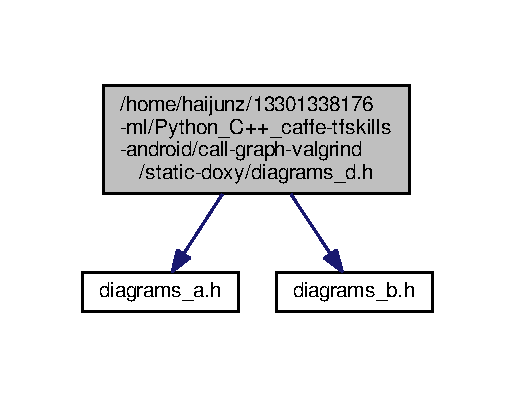
\includegraphics[width=247pt]{diagrams__d_8h__incl}
\end{center}
\end{figure}
This graph shows which files directly or indirectly include this file\-:\nopagebreak
\begin{figure}[H]
\begin{center}
\leavevmode
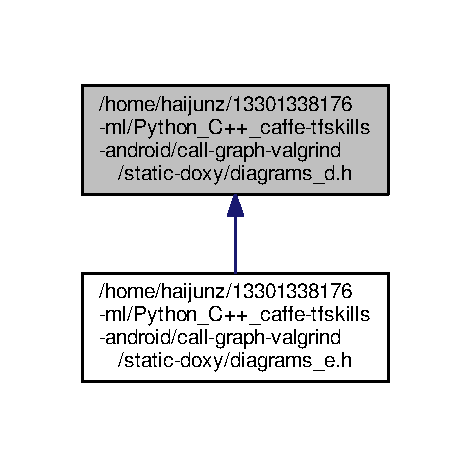
\includegraphics[width=226pt]{diagrams__d_8h__dep__incl}
\end{center}
\end{figure}
\subsection*{Classes}
\begin{DoxyCompactItemize}
\item 
class {\bf D}
\end{DoxyCompactItemize}

\section{/home/haijunz/13301338176-\/ml/\-Python\-\_\-\-C++\-\_\-caffe-\/tfskills-\/android/call-\/graph-\/valgrind/static-\/doxy/diagrams\-\_\-e.h File Reference}
\label{diagrams__e_8h}\index{/home/haijunz/13301338176-\/ml/\-Python\-\_\-\-C++\-\_\-caffe-\/tfskills-\/android/call-\/graph-\/valgrind/static-\/doxy/diagrams\-\_\-e.\-h@{/home/haijunz/13301338176-\/ml/\-Python\-\_\-\-C++\-\_\-caffe-\/tfskills-\/android/call-\/graph-\/valgrind/static-\/doxy/diagrams\-\_\-e.\-h}}
{\ttfamily \#include \char`\"{}diagrams\-\_\-d.\-h\char`\"{}}\\*
Include dependency graph for diagrams\-\_\-e.\-h\-:\nopagebreak
\begin{figure}[H]
\begin{center}
\leavevmode
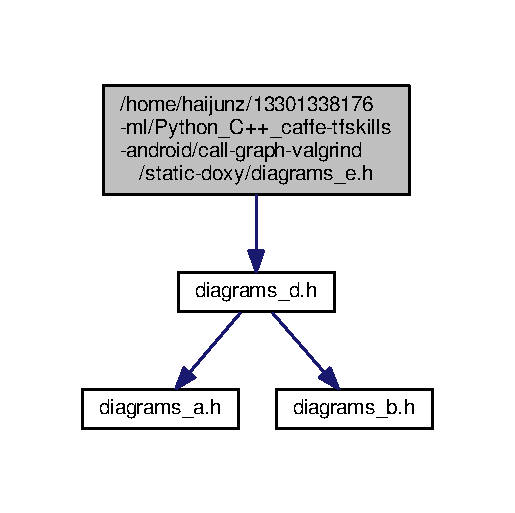
\includegraphics[width=247pt]{diagrams__e_8h__incl}
\end{center}
\end{figure}
\subsection*{Classes}
\begin{DoxyCompactItemize}
\item 
class {\bf E}
\end{DoxyCompactItemize}

\section{/home/haijunz/13301338176-\/ml/\-Python\-\_\-\-C++\-\_\-caffe-\/tfskills-\/android/call-\/graph-\/valgrind/static-\/doxy/\-R\-E\-A\-D\-M\-E.md File Reference}
\label{_r_e_a_d_m_e_8md}\index{/home/haijunz/13301338176-\/ml/\-Python\-\_\-\-C++\-\_\-caffe-\/tfskills-\/android/call-\/graph-\/valgrind/static-\/doxy/\-R\-E\-A\-D\-M\-E.\-md@{/home/haijunz/13301338176-\/ml/\-Python\-\_\-\-C++\-\_\-caffe-\/tfskills-\/android/call-\/graph-\/valgrind/static-\/doxy/\-R\-E\-A\-D\-M\-E.\-md}}

%--- End generated contents ---

% Index
\newpage
\phantomsection
\addcontentsline{toc}{chapter}{Index}
\printindex

\end{document}
